\begin{homeworkProblem}
A massless spring has unstretched length \( l_0 \) and force constant \( k \). One end is now attached to the ceiling and a mass \( m \) is hung from the other. The equilibrium length of the spring is now \( l_1 \).

\begin{enumerate}[(a)]
    \item Write down the condition that determines \( l_1 \).
        \begin{callout}{Solution:}
            
            The condition for equilibrium is simply that 
            $$m \textbf{F}=\textbf{a} = 0, \quad \stackrel{\textbf{F}=-kx + mg}{\implies} \quad 0 = -k(l_1-l_0) + mg$$
            Where $l_1$ would be the new equilibrium position. 
            $$l_1 = l_0 + \frac{mg}{k}$$
        \end{callout}
    \item Suppose now the spring is stretched a further distance \( x \) beyond its new equilibrium length. Show that the net force (spring plus gravity) on the mass is \( F = -kx \). That is, the net force obeys Hooke's law when \( x \) is the distance from the equilibrium position—a very useful result, which lets us treat a mass on a vertical spring just as if it were horizontal.
        \begin{callout}{Solution:}
            
            If we consider the motion to be one dimensional in a perfectly vertical axis, we have
            $$F = 0 = -k(l_1 - l_0) - mg$$
            Now if we find equilibrium position by setting net force to zero, 
            $$l_0-\frac{mg}{k} = l_1$$
            If we consider some displacement from this position $x$, we expect $mg$ to cancel:
            $$F = -k(x+l_1 -l_0)-mg = -kx$$

        \end{callout}
    \item Prove the same result by showing that the net potential energy (spring plus gravity) has the form \( U(x) = \text{const} + \frac{1}{2}kx^2 \).
        \begin{callout}{Solution:}
           
            \[ U(x) = mgh + \frac{1}{2}k(\alpha - l_0)^2 \]
            where $h$ is measured from some arbitrary reference level. If we choose our coordinate system such that $x = 0$ at equilibrium, then:
            \[ h = h_0 + x, \quad \alpha = l_1 + x \]
            where $h_0$ and $l_1$ correspond to the equilibrium position. Substituting:
            \[ U = mg(h_0 + x) + \frac{1}{2}k(l_1 + x - l_0)^2 \]
            At equilibrium, 
            \[ \frac{mg}{k} = l_1 - l_0. \]
            Using this and expanding the squared term:
            \[ U = mgh_0 + mgx + \frac{1}{2}k\big[(l_1 - l_0)^2 + 2(l_1 - l_0)x + x^2\big] \]
            \[ = mgh_0 + mgx + \frac{1}{2}k\left(\frac{mg}{k}\right)^2 + mgx + \frac{1}{2}kx^2 \]
            \[ = \big[mgh_0 + \frac{1}{2}k\left(\frac{mg}{k}\right)^2\big] + \frac{1}{2}kx^2 \]
            The term in square brackets is constant, giving us:
            \[ U = \text{const} + \frac{1}{2}kx^2 \]
            This quadratic form of the potential energy immediately implies that the restoring force
            \[ F = -\frac{dU}{dx} = -kx, \]
        \end{callout}
\end{enumerate}
\end{homeworkProblem}

\begin{homeworkProblem}
The potential energy of two atoms in a molecule can sometimes be approximated by the Morse function,
\[
U(r) = A \left[ \left( e^{(R-r)/S} - 1 \right)^2 - 1 \right],
\]
where \( r \) is the distance between the two atoms and \( A, R, \) and \( S \) are positive constants with \( S \ll R \).

\begin{enumerate}
    \item Sketch this function for \( 0 < r < \infty \).
        
        \begin{callout}{Solution:}
            \begin{center}
                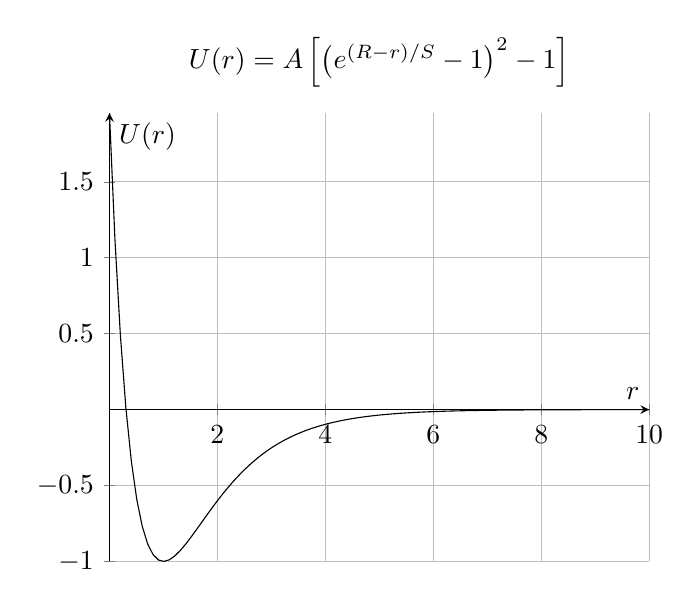
\begin{tikzpicture}
                    \begin{axis}[
                            xlabel={$r$},
                            ylabel={$U(r)$},
                            title={$U(r) = A \left[ \left( e^{(R-r)/S} - 1 \right)^2 - 1 \right]$},
                            axis lines=middle,
                            grid=both
                        ]
                        \addplot[domain=0:10,samples=100] {1*((exp((1-x)/1)-1)^2 - 1)};
                    \end{axis}
                \end{tikzpicture}
            \end{center}
       \end{callout} 

    \item Find the equilibrium separation \( r_0 \), at which \( U(r) \) is minimum.
        \begin{callout}{Solution:}

            \begin{align*}
                U(r) &= A\left(e^{2\left(R-r\right)/S}-2e^{(R-r)/S}\right) \\ 
                \nabla U(r) &= \frac{A}{S} \left(2e^{(R-r)/S}-2e^{2\left(R-r\right)/S}\right)
            \end{align*}
            
            Equilibrium for a potential function is when the function is at a minima or maxima

            \begin{align*}
                \nabla U(r) = 0 &= \frac{A}{S} \left(2e^{(R-r)/S}-2e^{2\left(R-r\right)/S}\right) \\
                r &= R
            \end{align*}
        \end{callout}
    \item Now write \( r = r_0 + x \) so that \( x \) is the displacement from equilibrium, and show that, for small displacements, \( U \) has the approximate form \( U = \text{const} + \frac{1}{2}kx^2 \). That is, Hooke's law applies. What is the force constant \( k \)?
        \begin{callout}{Solution:}
            
            $$e^{x/S}\approx 1 + \frac{x}{S} + \frac{x^2}{2S^2} + \dots$$
            \begin{align*}
                U(r) &= A \left[\left( 1 + \frac{[R-(r_0+x)]}{S} -1 \right)^2-1\right] \\ 
                &= A\left(\frac{[R-(r_0+x)]^2}{S^2}-1\right)
            \end{align*}
            Which is a quadratic potential with some vertical offset. If $S \ll R$, then the leading term should dominate. We could say that $k= \frac{2A}{S^2}$ such that we have an approximate potential where $x$ is the displacement from the equilibrium
            $$U(r)= \frac{1}{2}kx^2$$

        \end{callout}
\end{enumerate}
\end{homeworkProblem}

\begin{homeworkProblem}
The maximum displacement of a mass oscillating about its equilibrium position is \( 0.2 \, \mathrm{m} \), and its maximum speed is \( 1.2 \, \mathrm{m/s} \). What is the period \( \tau \) of its oscillations?
\begin{callout}{Solution:}
    \begin{align*}
        x(t) &= A\cos(\omega t + \delta) \\ 
        \dot{x}(t) &= - A \omega \sin (\omega t + \delta) \\ 
        \dot{x}_{max} &= A \omega && \text{maximized when $\sin(\omega t + \delta) = \pm1$} \\
        \omega &=  \frac{\dot{x}_{max}}{A} \\
        \tau &=  \frac{2\pi A}{\pi \dot{x}_{max}} && \text{$\tau = \frac{2\pi}{\omega}$ for sinusoidal motion} \\
        &= \frac{\pi}{3} \approx 1.05
    \end{align*}
\end{callout}
\end{homeworkProblem}

\begin{homeworkProblem}
Consider a particle in two dimensions, subject to a restoring force of the form (5.21). (The two constants \( k_x \) and \( k_y \) may or may not be equal; if they are, the oscillator is isotropic.) Prove that its potential energy is
\[
U = \frac{1}{2} \left( k_x x^2 + k_y y^2 \right).
\]
\begin{callout}{Solution:}
    We have forces
    $$\textbf{F} = \begin{pmatrix} -k_x x \\ -k_yy \end{pmatrix}$$
    We can use familiar techniques to get to a potential function
    \begin{align*}
        U &= \int -k_x x ~dx = -\frac{1}{2}k_x x^2 - k_y c(y) \\ 
        F_{y} &= \frac{dU}{dy} \implies -k_y y = -k_y c_y(y) \\ 
        c(y) &= \frac{1}{2}k_y y \\ 
        \textbf{F} = -\nabla U \quad \implies\quad  U &= \frac{1}{2}k_xx^2 + \frac{1}{2}k_yy^2
    \end{align*}
\end{callout}
\end{homeworkProblem}

\begin{homeworkProblem}
A damped oscillator satisfies the equation (5.24), where $F_{\mathrm{dmp}}=-b \dot{x}$ is the damping force. Find the rate of change of the energy $E=\frac{1}{2} m \dot{x}^2+\frac{1}{2} k x^2$ (by straightforward differentiation), and, with the help of (5.24), show that $d E / d t$ is (minus) the rate at which energy is dissipated by $F_{\text {dmp }}$.
\begin{callout}{Solution:}
    Differentiating non-damped energy, we get
    $$\frac{dE}{dt} = m\dot{x}\ddot{x} + k x \dot{x} = \dot{x} (m\ddot{x}+kx) $$
    Meanwhile
    $$F=m \textbf{a} = F_{dmp} \quad \to \quad m \ddot{x} = -b\dot{x} - kx$$
    where we have $F_{dmp}=-bdx / dt$.
    $$ E=\frac{m}{2}\left(\frac{d x}{d t}\right)^2+\frac{k}{2} x^2 . $$
    $$ \frac{d E}{d t}=\left(m \frac{d^2 x}{d t^2}+k x\right) \frac{d x}{d t}=-b \frac{d x}{d t}\left(\frac{d x}{d t}\right)=F_{d m p} \frac{d x}{d t}, $$

\end{callout}
\end{homeworkProblem}
